%
% This is the LaTeX template file for lecture notes for EE 382C/EE 361C.
%
% To familiarize yourself with this template, the body contains
% some examples of its use.  Look them over.  Then you can
% run LaTeX on this file.  After you have LaTeXed this file then
% you can look over the result either by printing it out with
% dvips or using xdvi.
%
% This template is based on the template for Prof. Sinclair's CS 270.

\documentclass[twoside]{article}
\usepackage{graphics}
\setlength{\oddsidemargin}{0.25 in}
\setlength{\evensidemargin}{-0.25 in}
\setlength{\topmargin}{-0.6 in}
\setlength{\textwidth}{6.5 in}
\setlength{\textheight}{8.5 in}
\setlength{\headsep}{0.75 in}
\setlength{\parindent}{0 in}
\setlength{\parskip}{0.1 in}

%
% The following commands set up the lecnum (lecture number)
% counter and make various numbering schemes work relative
% to the lecture number.
%
\newcounter{lecnum}
\renewcommand{\thepage}{\thelecnum-\arabic{page}}
\renewcommand{\thesection}{\thelecnum.\arabic{section}}
\renewcommand{\theequation}{\thelecnum.\arabic{equation}}
\renewcommand{\thefigure}{\thelecnum.\arabic{figure}}
\renewcommand{\thetable}{\thelecnum.\arabic{table}}

%
% The following macro is used to generate the header.
%
\newcommand{\lecture}[4]{
   \pagestyle{myheadings}
   \thispagestyle{plain}
   \newpage
   \setcounter{lecnum}{#1}
   \setcounter{page}{1}
   \noindent
   \begin{center}
   \framebox{
      \vbox{\vspace{2mm}
    \hbox to 6.28in { {\bf EE 382C/361C: Multicore Computing
                        \hfill Fall 2016} }
       \vspace{4mm}
       \hbox to 6.28in { {\Large \hfill Lecture #1: #2  \hfill} }
       \vspace{2mm}
       \hbox to 6.28in { {\it Lecturer: #3 \hfill Scribe: #4} }
      \vspace{2mm}}
   }
   \end{center}
   \markboth{Lecture #1: #2}{Lecture #1: #2}
   %{\bf Disclaimer}: {\it These notes have not been subjected to the
   %usual scrutiny reserved for formal publications.  They may be distributed
   %outside this class only with the permission of the Instructor.}
   \vspace*{4mm}
}

%
% Convention for citations is authors' initials followed by the year.
% For example, to cite a paper by Leighton and Maggs you would type
% \cite{LM89}, and to cite a paper by Strassen you would type \cite{S69}.
% (To avoid bibliography problems, for now we redefine the \cite command.)
% Also commands that create a suitable format for the reference list.
\renewcommand{\cite}[1]{[#1]}
\def\beginrefs{\begin{list}%
        {[\arabic{equation}]}{\usecounter{equation}
         \setlength{\leftmargin}{2.0truecm}\setlength{\labelsep}{0.4truecm}%
         \setlength{\labelwidth}{1.6truecm}}}
\def\endrefs{\end{list}}
\def\bibentry#1{\item[\hbox{[#1]}]}

%Use this command for a figure; it puts a figure in wherever you want it.
%usage: \fig{NUMBER}{SPACE-IN-INCHES}{CAPTION}
\newcommand{\fig}[3]{
			\vspace{#2}
    			\begin{center}
			Figure \thelecnum.#1:~#3
			\end{center}
	}
% Use these for theorems, lemmas, proofs, etc.
\newtheorem{theorem}{Theorem}[lecnum]
\newtheorem{lemma}[theorem]{Lemma}
\newtheorem{proposition}[theorem]{Proposition}
\newtheorem{claim}[theorem]{Claim}
\newtheorem{corollary}[theorem]{Corollary}
\newtheorem{definition}[theorem]{Definition}
\newenvironment{proof}{{\bf Proof:}}{\hfill\rule{2mm}{2mm}}

% **** IF YOU WANT TO DEFINE ADDITIONAL MACROS FOR YOURSELF, PUT THEM HERE:

\begin{document}
%FILL IN THE RIGHT INFO.
%\lecture{**LECTURE-NUMBER**}{**DATE**}{**LECTURER**}{**SCRIBE**}
\lecture{18}{October 27}{Vijay Garg}{Yu Sun}
%\footnotetext{These notes are partially based on those of Nigel Mansell.}

% **** YOUR NOTES GO HERE:

% Some general latex examples and examples making use of the
% macros follow.  
%**** IN GENERAL, BE BRIEF. LONG SCRIBE NOTES, NO MATTER HOW WELL WRITTEN,
%**** ARE NEVER READ BY ANYBODY.
\section{Atomic Scan}

Scan $\rightarrow$ Atomic read of multiple locations

Update $\rightarrow$ Atomic write of a single location
\newline
Assume the memory state is as following:

\centerline{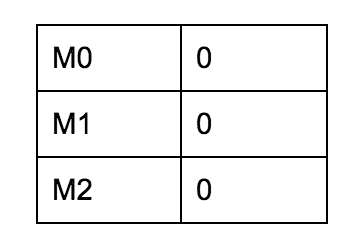
\includegraphics{memory.png}}

We now do two write operations:
write (M0, 1) and write (M1, 1)

It is possible that the scan return 010 which is not an atomic execution. Because read(M0) may happen before write(M0, 1) but read(M1) can happen after write(M1, 1).

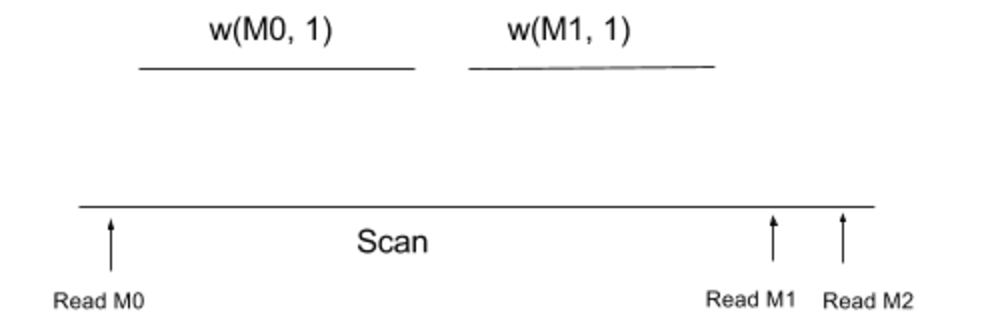
\includegraphics{scan.png}

\centerline{Non-atomic Scan}

\textbf{Solution}

So how to solve this problem? We add a timestamp to each value so that each write operation will update the corresponding timestamp and read operation can guarantee the consistency by compare the timestamps.

\textbf{Update}:
	Write the new value with updated timestamp.
	
\textbf{Scan}:
	Collect the entire array in W.
	
\textbf{Loop}:   
    Read the array again to make sure that there is no change in any timestamp.
    
If there is some change then go to Loop;

\section{Consensus}
The \textbf{consensus} problem requires a given set of processes to agree on an input value.

We abstract the consensus problem as follows: Each process has a value input to it that it can propose. For simplicity, we will restrict the range of input values to a single bit. The processes are required to run a protocol so that they decide on a common value.

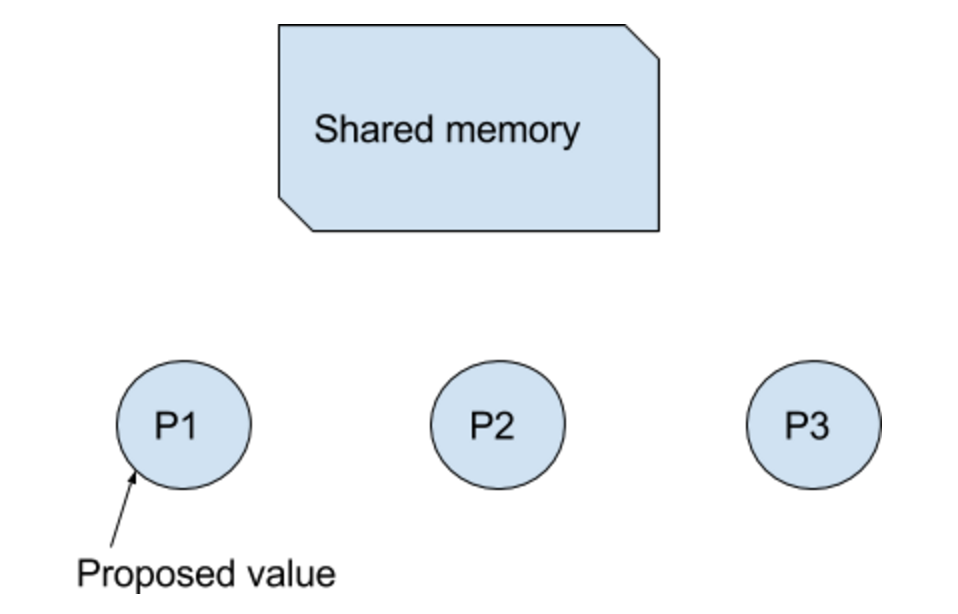
\includegraphics{consensus.png}

The \textbf{requirements} on any object implementing consensus are as follows:

\begin{itemize}
    \item Agreement:  No two correct processes decide on different values.
    \item Validity: The value decided must be proposed by some process.
    \item Wait-freedom: Decides in a finite number of steps.
\end{itemize}

A protocol is in a bivalent state if both the values are possible as decision values starting from that global state. 

A bivalent state is a critical state if all possible moves from that state result in nonbivalent states.

\subsection{Consensus Claims}

\textbf{Claim 1}: There exists an initial bivalent global state for any consensus protocol.

\textbf{Proof:}
Because there exist at least two runs from that state that result in different decision values. In the first run, the process with input 0 gets to execute and all other processes are very slow. Because of wait freedom, this process must decide, and it can decide only on 0 to ensure validity. A similar run exists for a process with its input as 1.

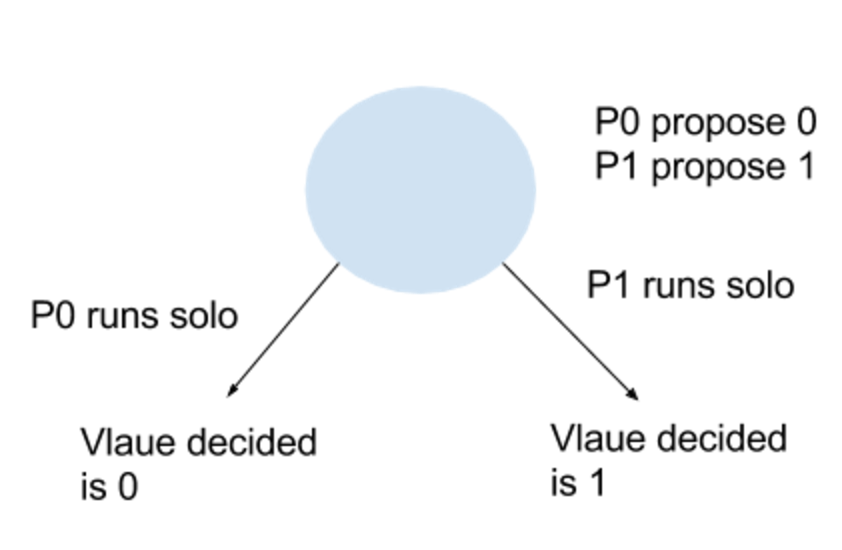
\includegraphics{proof1.png}

\textbf{Claim 2}: There exists a critical global state for every consensus protocol.

\textbf{Claim 3}: There does not exist any protocol to solve the consensus using atomic registers.
\textbf{Proof:} We show that even in a two-process system, atomic registers cannot be used to go to non-bivalent states in a consistent manner. We perform a case analysis of events that can be done by two processes, say, P and Q in a critical state S. Let e be the event at P and event f be at Q be such that e(S) has a decision value different from that of f(S). 
We now do a case analysis:

\centerline{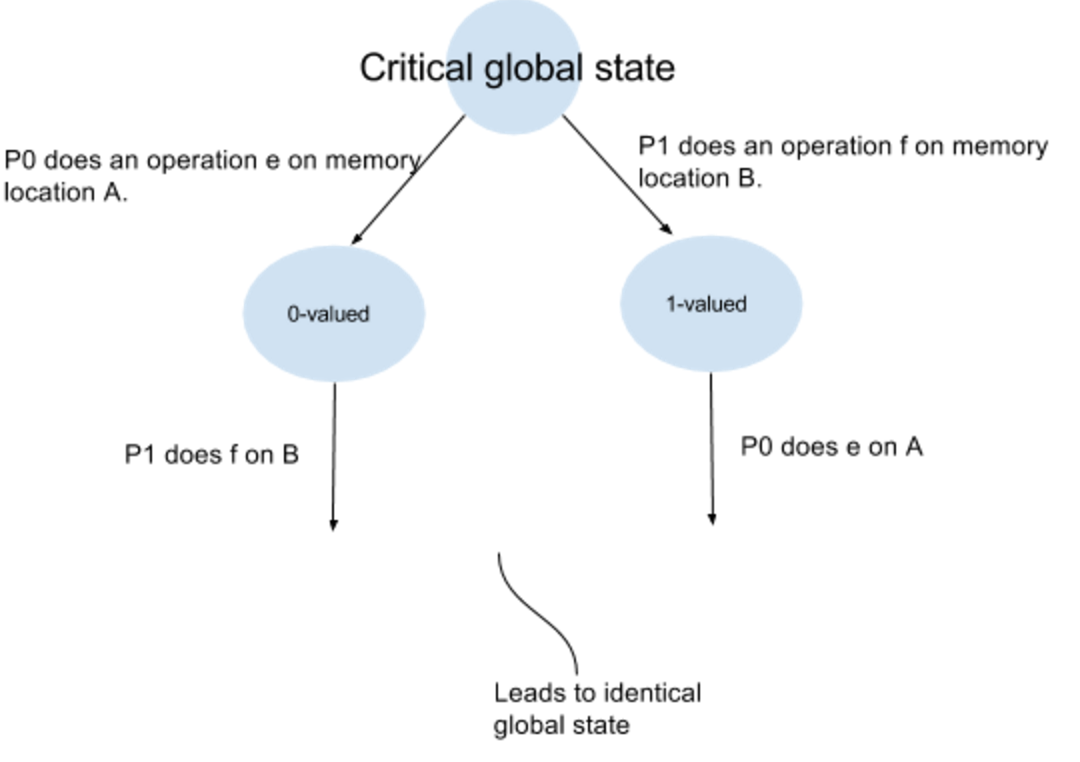
\includegraphics{case1.png}}

Case 1: e and f are on different registers. In this case, both ef and fe are possible in the critical state S. Further, the state ef(S) is identical to fe(S) and therefore cannot have different decision values. But we assumed that f(S) and e(S) have different decision values, which implies that e(f(S)) and f(e(S)) have different decision values because decision values cannot change.

\centerline{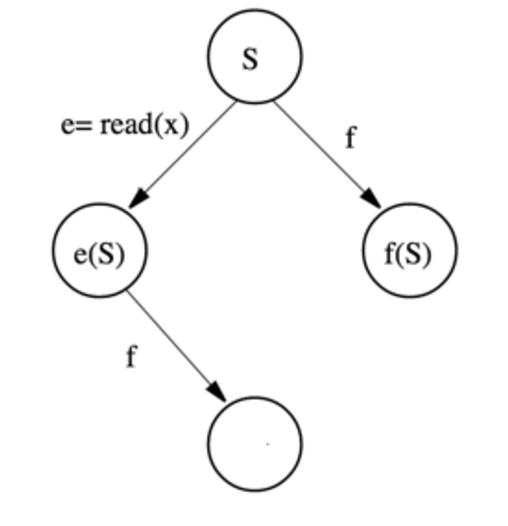
\includegraphics{case2.png}}

Case 2: Either e or f is a read. Assume that e is a read. Then the state of Q does not change when P does e. Therefore, the decision value for Q from f(S) and e(S), if it ran alone, would be the same; a contradiction.

\centerline{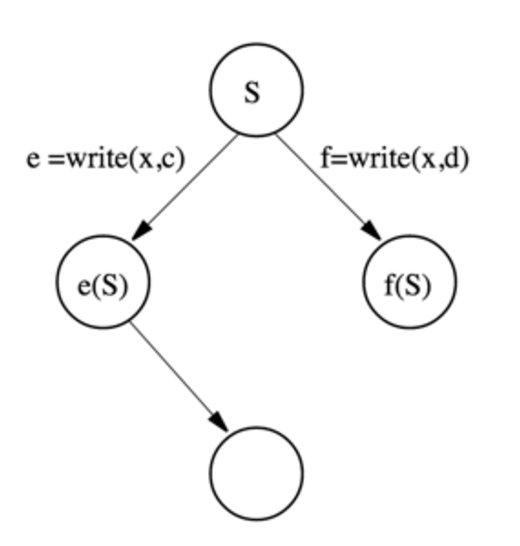
\includegraphics{case3.png}}

Case 3: Both e and f are writes on the same register. Again the states f(S) and f(e(S)) are identical for Q and should result in the same decision value.

\section{SPSC}

Assume we have a queue storing values of 'win' and 'lose'.

Pi:

\hspace{10mm} Write my proposal in the prop array.
    
\hspace{10mm} Deq from Queue 
    
\hspace{10mm} If I win choose my proposal, otherwise choose other guy’s proposal.
    

\textbf{Theorem}: There is no wait-free algorithm to build SPMC Queue using atomic read write registers.


\textbf{Proof}:
Consensus number of a shared object class O is the maximum number of processes that can use objects from class O to solve consensus.

\textbf{Consensus number} of a shared is the maximum number of processes that can use that object to solve consensus. The following is the operation with its corresponding consensus number.

Operation: Consensus Number

R/W Register: 1

Test And Set: 1

Get And Increment: 2

Swap: 2

CAS: $\infty$


\textbf{CAS Operation}

Initialize to -1

Pi:

\hspace{10mm} Write my proposal in the prop array

\hspace{10mm} Do R.CAS(-1, my\textunderscore pid):

\hspace{20mm} Fail: decide prop[R];
	
\hspace{20mm} Succeed: decide prop[my\textunderscore id];
	

\section*{References}
\beginrefs
\bibentry{1}{\sc V. K. ~Garg},
 Introduction to Multicore Computing
\endrefs


\end{document}





